\documentclass[12pt,a4paper]{article}
\usepackage[utf8]{inputenc}
\usepackage[german]{babel}
\usepackage{amsmath}
\usepackage{amsfonts}
\usepackage{amssymb}
\usepackage{graphicx}
\usepackage{amsmath}
\author{Moritz}
\usepackage[left=2cm,right=2cm,top=2cm,bottom=2cm]{geometry}
\begin{document}
	


	\subsubsection{Versuchsauswertung}
	
	Zunächst wurden die einzelnen Messreihen (Abbildung \ref{pic:messreihen_laufzeit}) gemittelt und auf statistische Fehler untersucht (Tabelle 1).
	\begin{figure}
	\begin{center}
		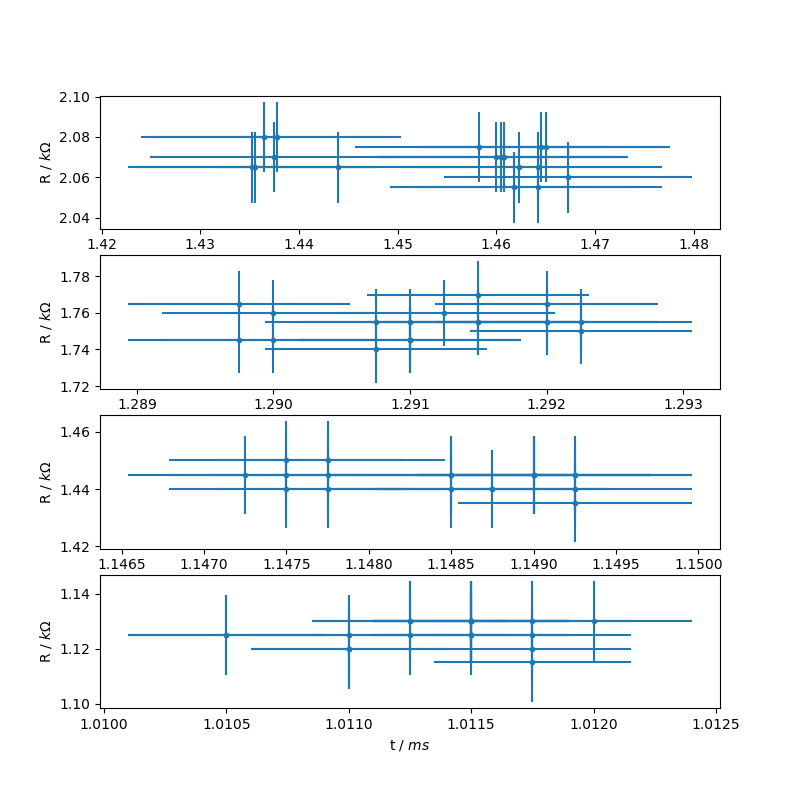
\includegraphics[width=0.5\linewidth]{messreihen_2bis5_laufzeit}
		\caption{Messreihen 2 bis 5 von insgesamt sieben Messreihen}
		\label{pic:messreihen_laufzeit}
	\end{center}
	\end{figure}
	\begin{table}
		\begin{center}
			\begin{tabular}{|c|c|}
				\hline
				\textbf{Widerstand [$k\Omega$]} & \textbf{Laufzeit [$ms$]} \\
				\hline
				2.3792 $\pm$ 0.0024 & 1,5914 $\pm$ 0,0017\\
				\hline
				2.0682 $\pm$ 0.0019 & 1,4534 $\pm$ 0,0030\\
				\hline
				1.7535 $\pm$ 0.0019 & 1,2911 $\pm$ 0,0018\\
				\hline
				1.4435 $\pm$ 0.0011& 1,1485 $\pm$ 0,0002\\
				\hline
				1.1260 $\pm$ 0.0012& 1,0114 $\pm$ 0,0001\\
				\hline
				0.8178 $\pm$ 0.0013& 0,8721 $\pm$ 0,0001 \\
				\hline
				0.5075 $\pm$ 0.0011&  0,7338 $\pm$ 0,0001 \\
				\hline
			\end{tabular}
		\end{center}
		\caption{Mittelwerte der Messreihen mit stat. Fehlern}
	\end{table}	
	\begin{figure}
	\begin{center}	
		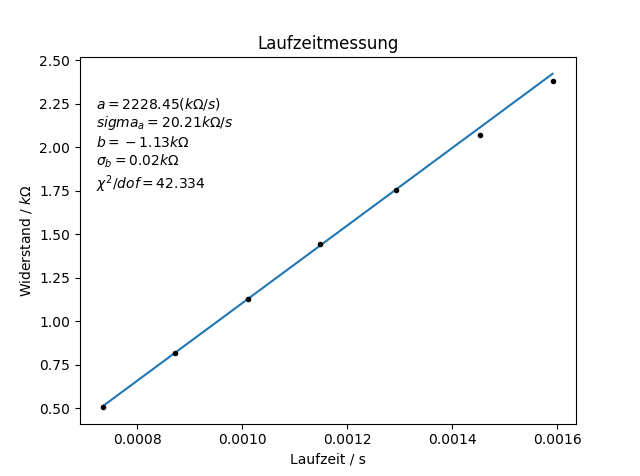
\includegraphics[width=0.6\linewidth]{fit_laufzeit}
		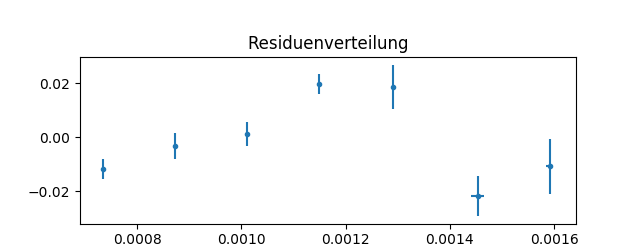
\includegraphics[width=0.6\linewidth]{residuen_laufzeit}
		\caption{Mittelwerte der Messreihen mit angepasster Geraden durch die Messwerte}
		\label{pic:fit_laufzeit}
		
		
	\end{center}
	\end{figure}
	An alle Messreihen zusammen wurde eine Gerade angepasst (Abbildung \ref{pic:fit_laufzeit}), es ergab sich für deren Steigung:
	\begin{equation}
	\frac{\Delta R}{\Delta t} = (2228,45 \pm 20,21) \frac{k\Omega}{s}
	\end{equation} 
	Gesucht ist die Schallgeschwindigkeit $v_{Schall}$, diese ergibt sich als Steigung der Geraden an die Messwerte, wobei die Widerstände noch in Entfernungen umgerechnet werden müssen. Da nur die Steigung von Interesse ist und nicht der y-Achsenabschnitt, wurde die tatsächliche  Entfernung Lautsprecher - Mikrofon weder gemessen noch berechnet. Es gilt:
	
	\begin{equation}
	v_{Schall} = \frac{\Delta s}{\Delta t} = \frac{\Delta s}{\Delta R} \cdot \frac{\Delta R}{\Delta t} = k \frac{\Delta R}{\Delta t} = 356,33 \frac{m}{s}
	\end{equation}
	\begin{equation}
	\sigma_{stat} = v_{Schall} \frac{\sigma _{\Delta R / \Delta t}}{\Delta R / \Delta t} = 3,23 \frac{m}{s}
	\end{equation}
	\begin{equation}
	\sigma_{sys} = v_{Schall} \frac{\sigma _k}{k} = 1,56 \frac{m}{s}
	\end{equation}
	
	Also erhält man als Ergebnis des Versuchs:
	\begin{equation}
	v_{Messung} = (356.33 \pm 3.232 \pm 1.56)\frac{m}{s} = (356,33\pm 3,59) \frac{m}{s}
	\end{equation}
	Aus der Temperaturmessung erhielten wir, dass die Raumtemperatur zu Beginn des Versuchs $T = (23,6 \pm 1)C = (296,7 \pm 1)K$ betrug.
	Daraus ergibt sich eine Schallgeschwindigkeit von
	\begin{equation}
	v_{Theorie} =\sqrt{\frac{R\cdot\kappa}{M_mol}}\sqrt{T} = 345,14 \frac{m}{s} \text{\qquad mit \qquad}
	\sigma = 0,5 \sqrt{\frac{R\cdot\kappa}{M_mol}} \frac{\sigma_T}{\sqrt{T}} = 0,58 \frac{m}{s}
	\end{equation}
	Die Abweichung der Messung von der Theorie beträgt demnach 3.1 Standardabweichungen. Die relative Unsicherheit auf die Schallgeschwindigkeit beträgt 1\%.\\
	Das $\chi^2/dof=42,3$ zeigt, dass die sieben Mittelwerte nicht auf einer Geraden liegen. Außerdem sind die Fehler auf die Mittelwerte deutlich geringer als die Abweichungen von der Geraden. Allerdings ist unklar worin diese begründet ist, da der Versuchsaufbau und die Kalibration des Potentiometers nicht verändert wurden. Aus der Residuenverteilung ist zu erkennen, dass die fünf linken Werte etwa auf einer Geraden liegen. Beachtet man nur die fünf linken Werte, so erhält man mit $v_{links} = 359.354 m/s$ auch keinen besseren Wert für die Schallgeschwindigkeit.  Berechnet man die Schallgeschwindigkeit nur aus den rechten beiden Messungen (diese wurden zeitlich zuerst durchgeführt), so erhält man $v_{rechts} = 361.519 m/s$, einen noch schlechteren Wert.\\
	Außerdem ist auffällig, dass die ersten drei Werte deutlich größere Fehler aufweisen als die letzten vier Werte.
	

\end{document}